\documentclass[]{article}
\usepackage{circuitikz}
\usepackage{listings}
\usepackage{xcolor}
\usepackage{graphicx}
\definecolor{codegreen}{HTML}{859900}
\definecolor{codegray}{HTML}{839496}
\definecolor{codepurple}{HTML}{6C71C4}
\definecolor{codemagenta}{HTML}{d33682}
\definecolor{backcolour}{HTML}{FDF6E3}
\definecolor{fontcolor}{HTML}{002B36}
\lstdefinestyle{mystyle}{
	basicstyle=\color{fontcolor},
	backgroundcolor=\color{backcolour},   
	commentstyle=\color{codegreen},
	keywordstyle=\color{codemagenta},
	numberstyle=\tiny\color{codegray},
	stringstyle=\color{codepurple},
	breakatwhitespace=false,         
	breaklines=true,                 
	captionpos=b,                    
	keepspaces=true,                 
	numbers=left,                    
	numbersep=5pt,                  
	showspaces=false,                
	showstringspaces=false,
	showtabs=false,                  
	tabsize=4
}
\lstset{style=mystyle}
\title{Lab 8\\ADC}
\author{Keaton Clark}

\begin{document}
\maketitle
	\section*{Circuit}
		\begin{center}
			\begin{circuitikz}
				\draw (0,0) to
					[short, o-, l={$A_0$}](0,0) to
					[short, -](2,0)
				;
				\draw (0,2) to
					[short, o-, l={$5v$}](0,2) to
					[short, -](2,2)
				;
				\draw (2,2) to
					[phR](2,0) to
					[R,l={$330\Omega$}](2,-2) to
					(0,-2)node[ground, rotate=-90]
				;
			\end{circuitikz}
		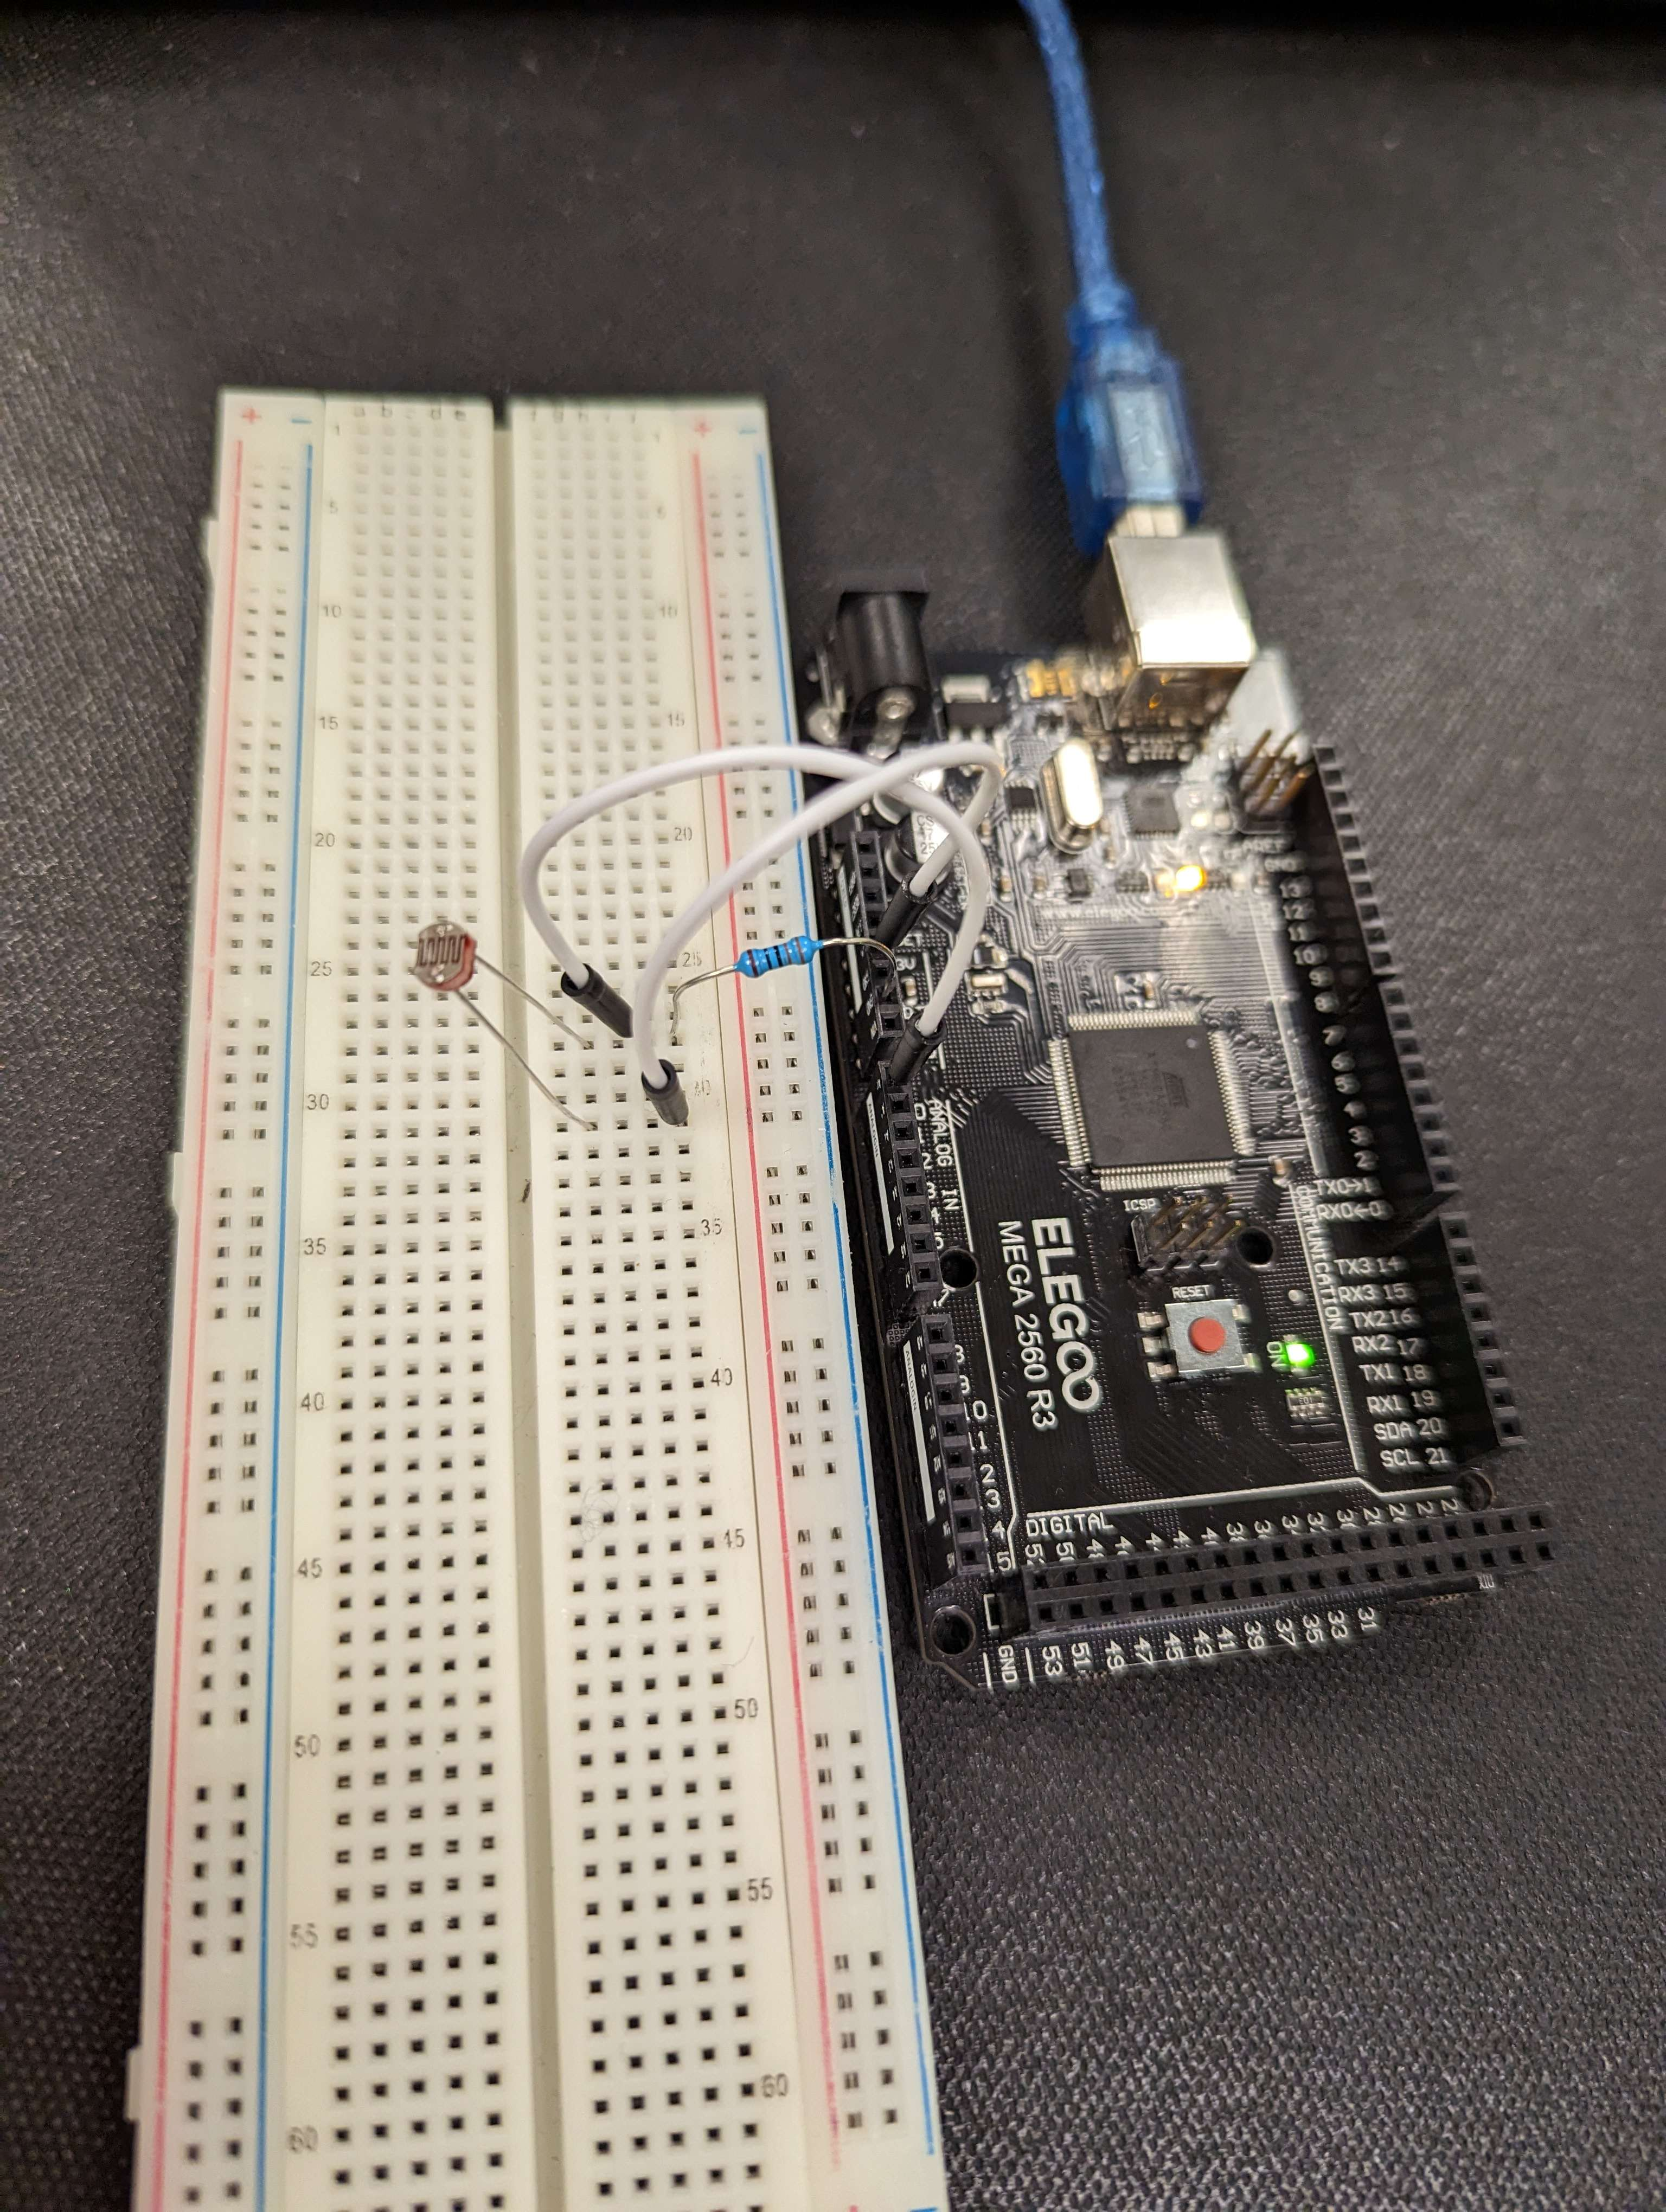
\includegraphics[width=\textwidth,angle=90]{./images/1.jpg}
		\end{center}
	\section*{Code}
		The modified code for part 3 is adding the if block on lines 15:19\\
		\lstinputlisting[language=C, caption={main.c}]{../src/main.c}
		\lstinputlisting[language=C, caption={io.h 241:253}, firstline=241, lastline=253, firstnumber=241]{../src/io.c}
	\section*{Results}
		\begin{center}
			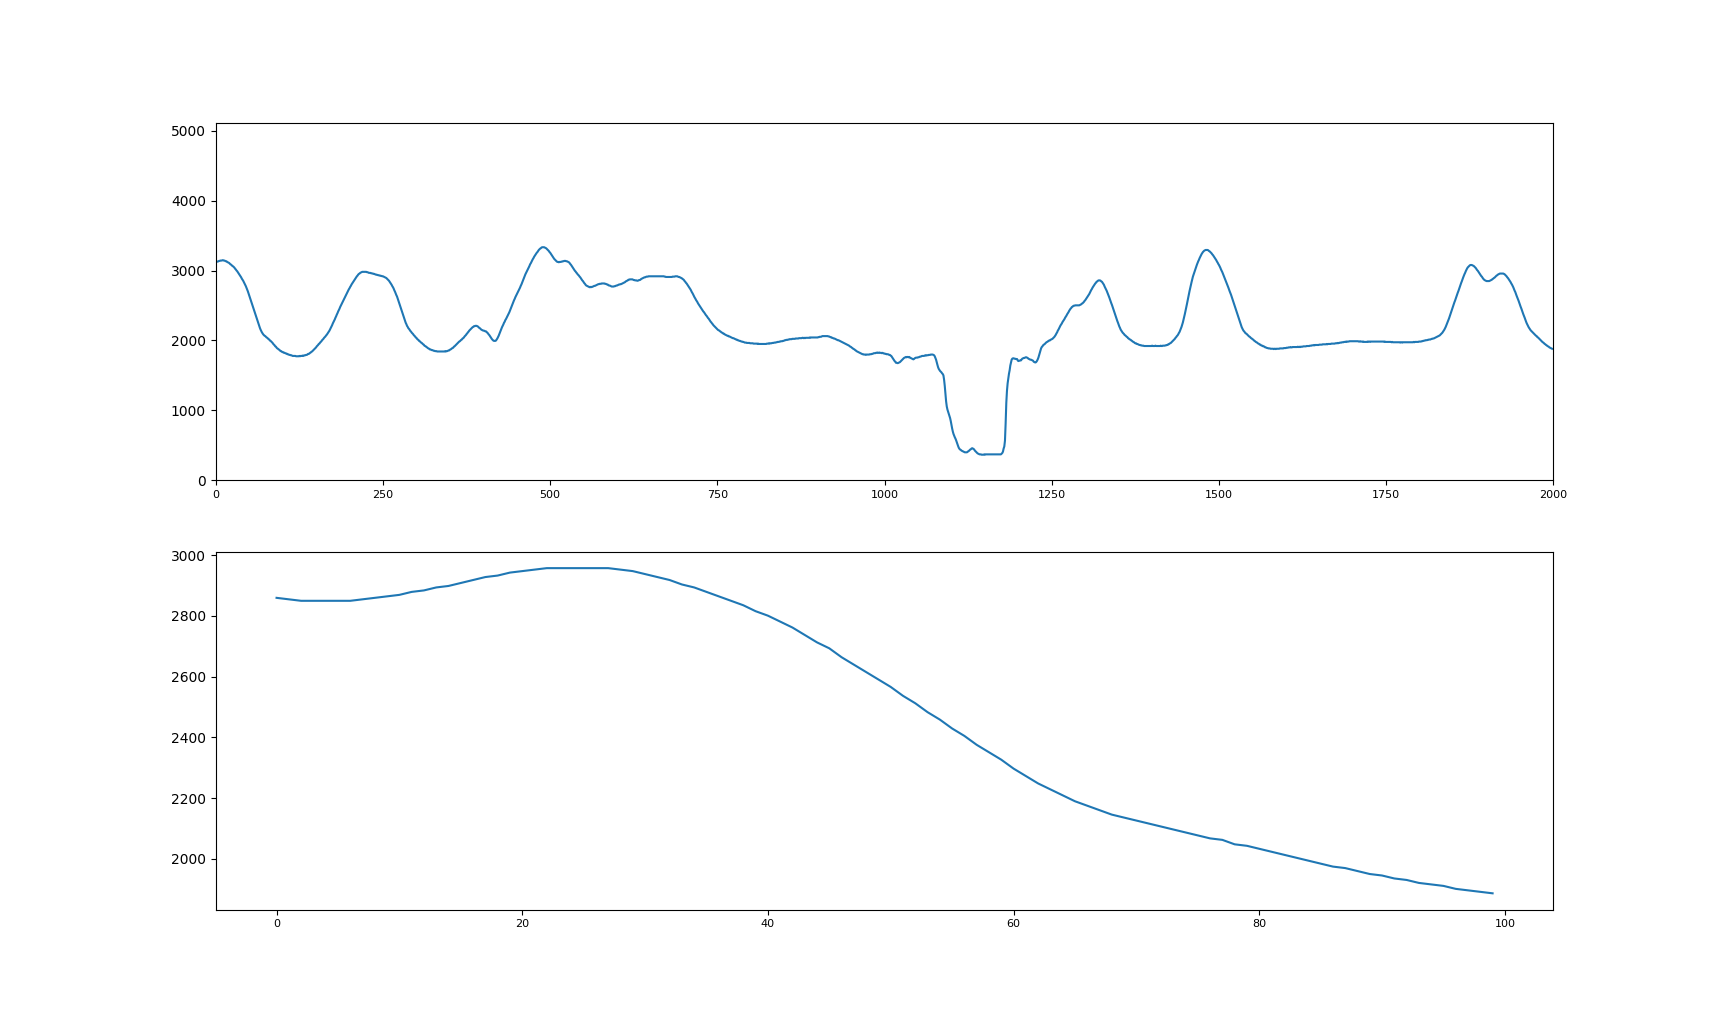
\includegraphics[width=\textwidth]{./images/1.png}
		\end{center}
\end{document}
